\vspace{1cm}
\fancyhead[C]{\normalsize\textbf{$\qquad$ Teil I: Offene Aufgaben}}
\renewcommand{\labelenumi}{\theenumi.}
\section*{Aufgabe 1 (36 Punkte)}
\vspace{0.4cm}
\section*{Aufgabe 1 (36 Punkte)}
\vspace{0.4cm}
%\titleformat{\subsection}[runin]
%{\normalfont\large\bfseries}{\thesubsection}{1em}{}
\subsection*{\aufgabe{a1}{6}} 
Thomas Robert Malthus (1766-1834), ein britischer Ökonom und Pfarrer, veröffentlichte
1798 seinen vielbeachteten \textit{Essay on the Principle of Population}.
Er formulierte das Axiom, dass die Weltbevölkerung exponentiell wachse, die Nahrung dagegen nur linear. 
Das bedeutet, dass die Funktion $ n(t) $, welche die Anzahl Menschen angibt, die man bei optimaler Verteilung der zur Verfügung stehenden Nahrungsmittel zu Zeit $ t $ ernähren könnte, eine lineare ist:
\begin{align*}
	n(t) = a + b \cdot t.
\end{align*}
Die Weltbevölkerung $ w(t) $ betrug im Jahre 1800 ($ t= 0 $) rund eine Milliarde, d.h. $ w(0) = 10^9 $.
Wir wollen annehmen, dass die Weltbevölkerung rund $ 1\% $ pro Jahr wächst.
Außerdem wollen wir mit
\begin{align*}
	a = 2 \cdot 10^9 \ \textrm{und} \ b = 0.2 \cdot 10^9
\end{align*}
rechnen.
\begin{description}
	\item[Beweisen Sie:] 
	Es gibt genau einen Zeitpunkt $ t^\star > 400 $, an dem die Weltbevölkerung gerade noch ernährt werden kann, d.h., für $ w(t^\star)  = n(t^\star )$ ist.
\end{description}  
\
\\
\textbf{Lösung:}
\begin{mdframed}
\underline{\textbf{Vorgehensweise:}}
\renewcommand{\labelenumi}{\theenumi.}
\begin{enumerate}
\item 

\end{enumerate}
\end{mdframed}
\underline{1. }\\

 


\newpage

\subsection*{\aufgabe{a2}{6}}
Thomas Robert Malthus (1766-1834), ein britischer Ökonom und Pfarrer, veröffentlichte
1798 seinen vielbeachteten \textit{Essay on the Principle of Population}.
Er formulierte das Axiom, dass die Weltbevölkerung exponentiell wachse, die Nahrung dagegen nur linear. 
Das bedeutet, dass die Funktion $ n(t) $, welche die Anzahl Menschen angibt, die man bei optimaler Verteilung der zur Verfügung stehenden Nahrungsmittel zu Zeit $ t $ ernähren könnte, eine lineare ist:
\begin{align*}
	n(t) = a + b \cdot t.
\end{align*}
Die Weltbevölkerung $ w(t) $ betrug im Jahre 1800 ($ t= 0 $) rund eine Milliarde, d.h. $ w(0) = 10^9 $.
Wir wollen annehmen, dass die Weltbevölkerung rund $ 1\% $ pro Jahr wächst.
Außerdem wollen wir mit
\begin{align*}
	a = 2 \cdot 10^9 \ \textrm{und} \ b = 0.2 \cdot 10^9
\end{align*}
rechnen.\\
\\
Es gibt genau einen Zeitpunkt $ t^\star > 400 $, an dem die Weltbevölkerung gerade noch ernährt werden kann, d.h., für $ w(t^\star)  = n(t^\star )$ ist.\\
\\
Verwenden Sie eine Taylor-Approximation zweiter Ordnung im Punkt $ t_0 = 400 $, um eine Näherung für $ t^\star $ zu finden.
\\ \\
\textbf{Lösung:}
\begin{mdframed}
\underline{\textbf{Vorgehensweise:}}
\renewcommand{\labelenumi}{\theenumi.}
\begin{enumerate}
\item 
\end{enumerate}
\end{mdframed}

\underline{1. }\\


\newpage
\subsection*{\aufgabe{b}{10}}
Max hat über seine Verhältnisse gelebt. 
Deshalb hat er nun Schulden von mehreren hunderttausend Franken.
Die Schuldenberatung vermittelt ihm am Anfang des Jahres einen Privatkredit mit $ i = 5 \% $ in der genannten Höhe von $ S = 355'000 \ [\textrm{CHF}] $, den er in $ 12 $ gleich grossen Raten $ C $ jeweils per Jahresende abbezahlen muss. 
\begin{enumerate}
	\item[(b1)] Fügen Sie die Ereignisse und Mittelflüsse dem Zeitstrahl hinzu.
	\item[(b2)] Berechnen Sie die Höhe der Ratenzahlung $ C $.
\end{enumerate}
Am Ende des vierten Jahres gewinnt Max im Lotto CHF $ 160'000 $.
Er beschließt in diesem Jahr statt der normalen Rate $ C $ den ganzen Lottogewinn zur Abzahlung des Kredits zu benützen.
\begin{enumerate}
	\item[(b3)] Ergänzen Sie die Information am Zeitstrahl und berechnen Sie die Restschuld $ \overline{S} $ nach der Einzahlung am Ende des vierten Jahres.
\end{enumerate}
Max zahlt nun weiter am Ende jeden Jahres den Betrag $ C $ zu Tilgung seiner Restschuld $ \overline{S} $.
\begin{enumerate}
	\item[(b4)] Wie viele Zahlungen muss er machen, bis er die Restschuld vollkommen getilgt hat?
	\item[(b5)] Mit der letzten Rate muss nicht mehr der komplette Betrag $ C $ geleistet werden. Wie hoch ist die Zahlung genau?
\end{enumerate}
\begin{center}
	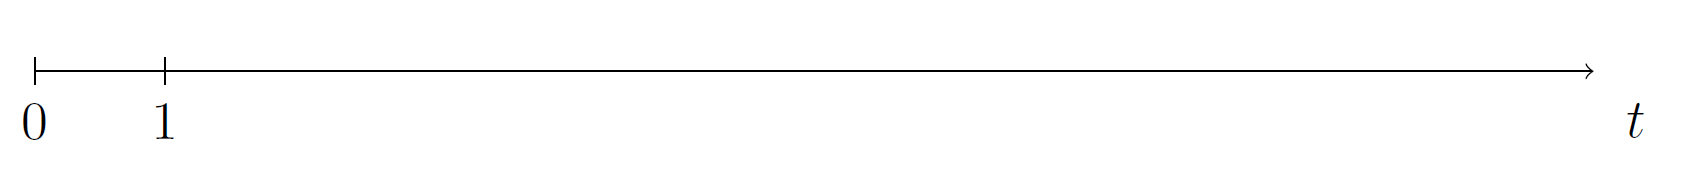
\includegraphics[scale=0.3]{pictures/zeitstrahl_1_b}
\end{center}
\ \\
\textbf{Lösung:}
\begin{mdframed}
\underline{\textbf{Vorgehensweise:}}
\begin{enumerate}
\item 
\end{enumerate}
\end{mdframed}

\underline{1. }\\



\newpage
\subsection*{\aufgabe{c}{6}}
Nach der Relativitätstheorie gilt für die Masse $ m $ eines Körpers, der sich mit der Geschwindigkeit $ v $ bewegt
\begin{align*}
	m(v)
	=
	\frac{m_0}{\sqrt{1 - \frac{v^2}{c^2}}}.
\end{align*}
Dabei ist $ c $ die Lichtgeschwindigkeit $ (299'792'458 \nicefrac{m}{s}) $ und $ m_0 $ die Masse in Ruhe.
\begin{enumerate}
	\item[(c1)] Berechnen Sie die Elastizität $ \varepsilon_m $ von $ m(v) $.
	\item[(c2)] Um wie viel Prozent ändert sich näherungsweise die Masse, wenn die Geschwindigkeit von $ v_0 = 0.5c $ um $ 5 \% $ erhöht wird?
\end{enumerate}
\ \\
\textbf{Lösung:}
\begin{mdframed}
\underline{\textbf{Vorgehensweise:}}
\begin{enumerate}
\item 
\end{enumerate}
\end{mdframed}

\underline{1.}\\


\newpage
\subsection*{\aufgabe{d}{8}}
Bei einer Absatzmenge $ x \geq 20  $ kann ein Monopolist mit dem Ertrag $ E(x) $ und den Kosten $ K(x) $ rechnen, die wie folgt gegeben sind:
\begin{align*}
	E(x) = -0.5 x^{1.5} +100 x \ \textrm{und} \ K(x) = -200\sqrt{x} + 50 x +120.
\end{align*}
Von seinem Bruttogewinn muss der Hersteller $ i \% $  $ (0 < i < 100) $ an Steuern bezahlen.
\begin{enumerate}
	\item[(d1)]
	Drücken Sie den Gewinn $ G(x) $ nach Steuern in Abhängigkeit der verkauften Menge $ x $ aus.
	\item[(d2)] 
	Für welche Menge $ x^\star $ maximiert der Hersteller seinen Gewinn nach Steuern?
\end{enumerate}
\ \\
\textbf{Lösung:}
\begin{mdframed}
	\underline{\textbf{Vorgehensweise:}}
	\begin{enumerate}
		\item[(d1)] 
	\end{enumerate}
\end{mdframed}


\underline{(d1) }\\





